% Adjust these for the path of the theme and its graphics, relative to this file
%\usepackage{beamerthemeFalmouthGamesAcademy}
\usepackage{../../beamerthemeFalmouthGamesAcademy}
\usepackage{multimedia}
\graphicspath{ {../../} }

% Default language for code listings
\lstset{language=C++,
        morekeywords={each,in,nullptr}
}

% For strikethrough effect
\usepackage[normalem]{ulem}
\usepackage{wasysym}
\usepackage{graphicx} %package to manage images

\usepackage{pdfpages}

% http://www.texample.net/tikz/examples/state-machine/
\usetikzlibrary{arrows,automata}


\newcommand{\modulecode}{COMP702}\newcommand{\moduletitle}{Classical Artificial Intelligence}\newcommand{\sessionnumber}{1}

\begin{document}
\title{\sessionnumber: Introduction to Design}
\subtitle{\modulecode: \moduletitle}

\frame{\titlepage} 

\part{Design Frameworks}
\frame{\partpage}

\begin{frame}{Iterative Game Design Process}
	\begin{figure}
		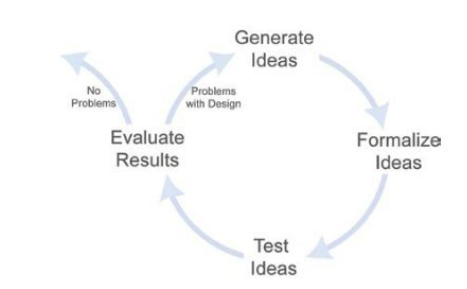
\includegraphics[width=1.0\textwidth,height=0.7\textheight]{iterative_game_design}
		\caption{taken from Game Design Workshop}
		\label{fig:iter1}
	\end{figure}
	\note[item]{Set player experience goals}
\end{frame}

%Set player experience goals
%Brainstorm ideas
%Build a prototype or document system/gameplay etc
%Test ideas (expert or audience)
%Evaluate results
%if idea doesn't work at all, start the process over
%if idea works, modify and test again

\begin{frame}{Design Thinking}
	\begin{figure}
		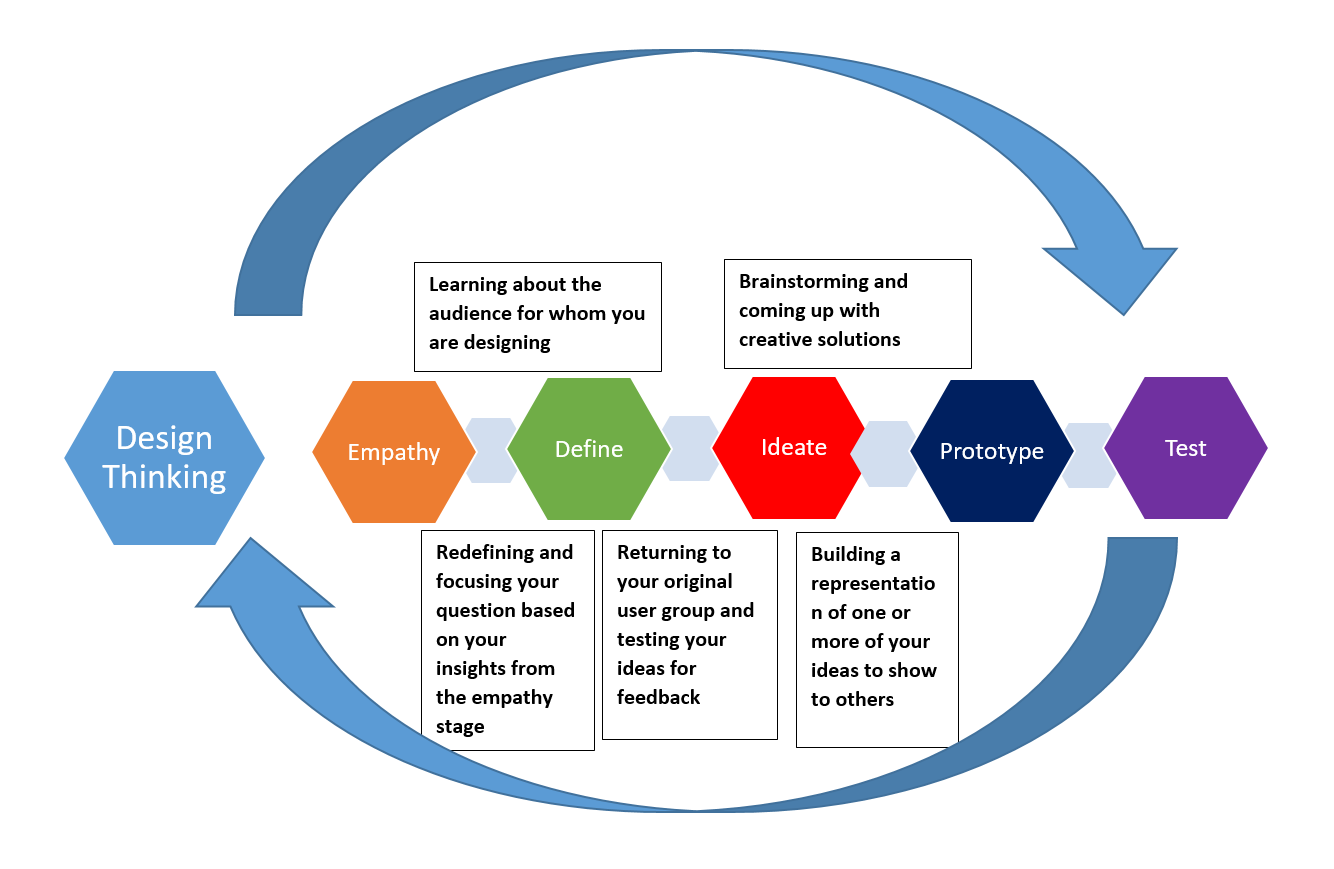
\includegraphics[width=1.0\textwidth, height=0.7\textheight]{design_thinking}
		\label{fig:design_thinking1}
	\end{figure}	
\end{frame}

%important to remember that you can jump around

\begin{frame}{Double Diamond}
	\begin{figure}
		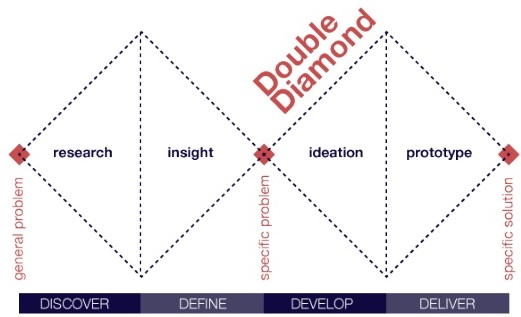
\includegraphics[width=1.0\textwidth, height=0.7\textheight]{double_diamond}
		\label{fig:double_diamond}
	\end{figure}
\end{frame}

%Created by the Design Council
%Discover. The first diamond helps people understand, rather than simply assume, what the problem is. It involves speaking to and spending time with people who are affected by the issues.
%Define. The insight gathered from the discovery phase can help you to define the challenge in a different way.
%Develop. The second diamond encourages people to give different answers to the clearly defined problem, seeking inspiration from elsewhere and co-designing with a range of different people. 
%Deliver. Delivery involves testing out different solutions at small-scale, rejecting those that will not work and improving the ones that will.

\begin{frame}{Summary}
\begin{itemize}
	\item Notice the key similarities in these models
	\item Iteration, testing and revising are key
	\item We are now going to look at tools to capture high level design choices
\end{itemize}
\end{frame}
\part{Design Goals}
\frame{\partpage}

\begin{frame}{Intro}
	\begin{itemize}
		\item As a designer it is important to have sort of intent
		\item It is important to think of what kind of response you want from your audience
		\item 
	\end{itemize}
\end{frame}

\begin{frame}{Design Pillars}
	\begin{itemize}
		\item Something about your game that everything should revolve around
		\item Establish once the your are in production
		\item Better for larger games
		\item Traditionally this is focused on mechanics but try to think about emotions you want at the core of your game
	\end{itemize}
\end{frame}

\begin{frame}{Audience/Player Experience Goals}
	\begin{itemize}
		\item Less rigid than Design Pillars
		\item You should focus on the emotional journey you want the player to go on
		\item This should inform your design process at all times
		\item If a feature detracts from this experience then cut it
	\end{itemize}
\end{frame}

\begin{frame}{Constraints}
	\begin{itemize}
		\item Constraints are drivers for creativity
		\item As a Designer you will bump up against them
		\item The Friction caused will cause you to think of ideas to beat the constraints
		\item Or to bend them to your will and use them in your design
	\end{itemize}
\end{frame}

\begin{frame}{Game Design Macro}
	\begin{itemize}
		\item Monolithic Design Docs are not very useful
		\item No-one in the team reads them
		\item Document is slow to evolve
		\item Game Design Macro attempts to capture the high level design 
	\end{itemize}
\end{frame}

\begin{frame}{Game Design Macro}
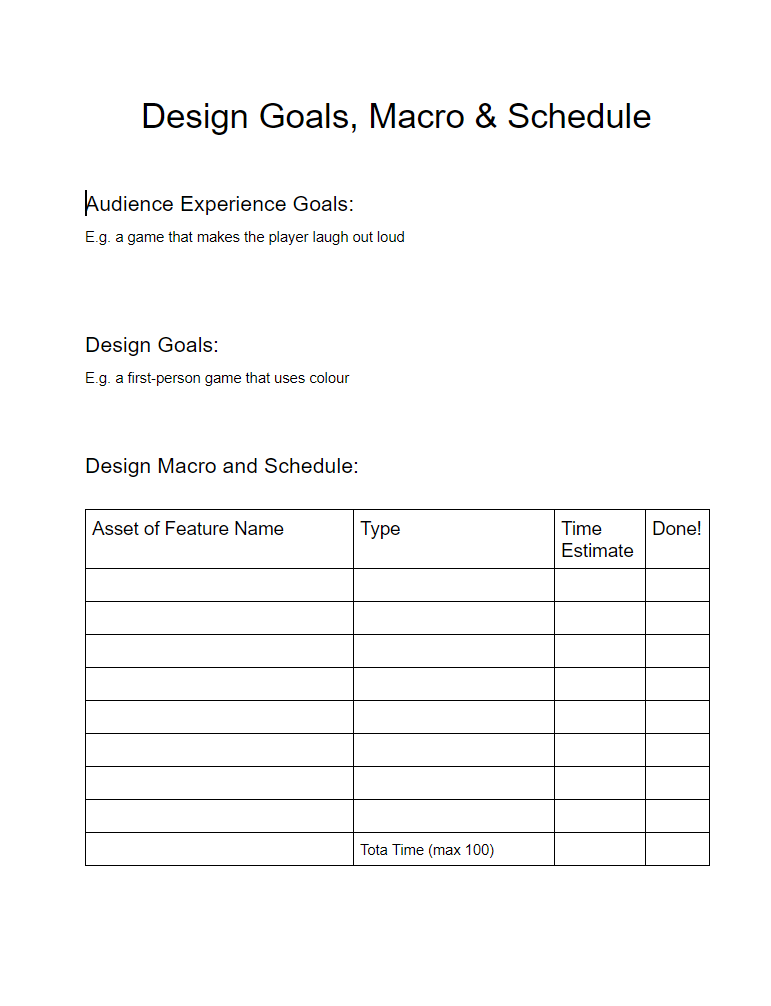
\includegraphics[width=1.0\textwidth]{game_design_macro}
\end{frame}

\begin{frame}{One Page Designs}
	\begin{itemize}
		\item First described by Stone Librande (Riot Games) 
		\item Instead of writing a Design Doc
		\item You write a series of one page design docs which detail some aspect of the game
		\item This could be a map, a visual description of the combat, relationship between characters
	\end{itemize}
\end{frame}

\begin{frame}{One Page Designs}
	\begin{center}
		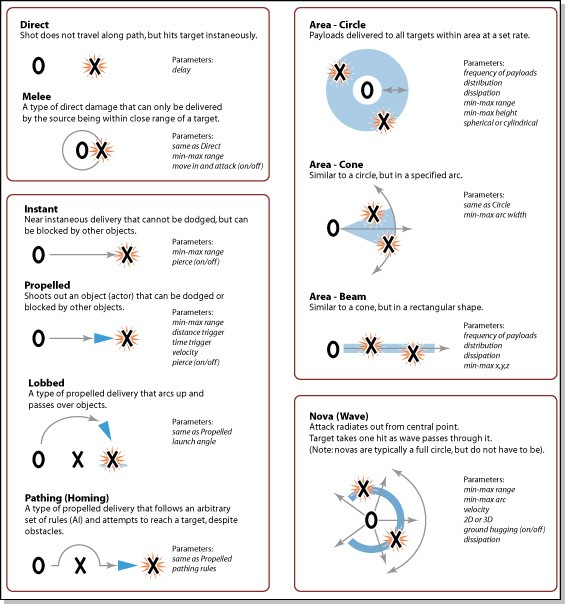
\includegraphics[width=0.7\textwidth,height=0.7\textheight]{combat_diagram}
	\end{center}
\end{frame}

\begin{frame}{One Page Designs}
	\begin{center}
		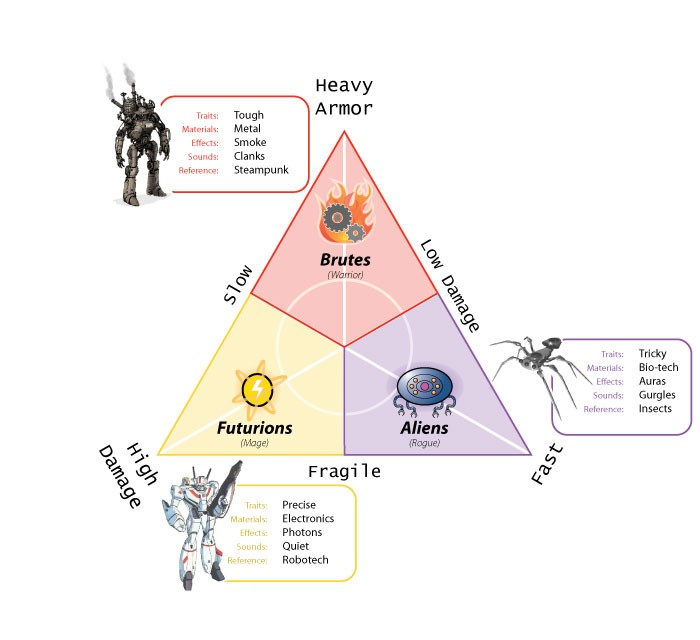
\includegraphics[width=0.7\textwidth,height=0.7\textheight]{unit_diagram}
	\end{center}
\end{frame}

\begin{frame}{One Page Design Template}
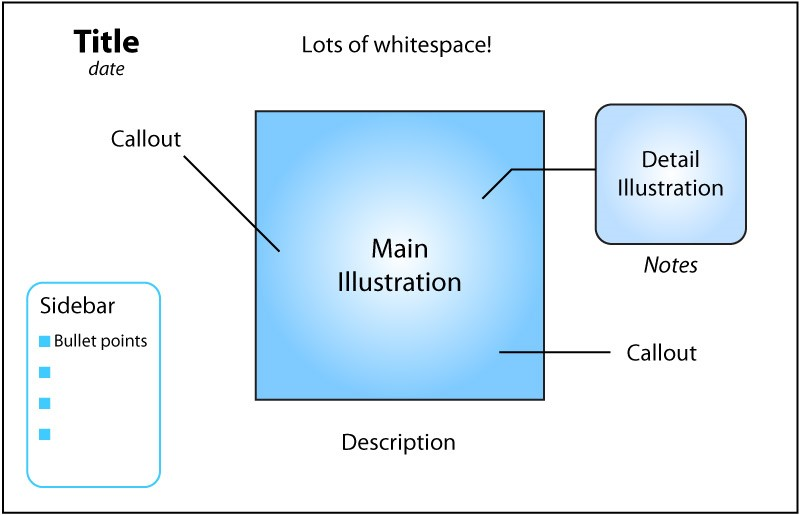
\includegraphics[width=1.0\textwidth]{one_page_design_template}
\end{frame}

\begin{frame}{One Page Design Benefits}
\begin{itemize}
	\item Forces a complete understanding of the game
	\item Forces a concise design
	\item Highlights relationships
	\item Aids problem solving
\end{itemize}
\end{frame}


\begin{frame}{References}
	\begin{itemize}
		\item Fullerton, T., 2018. Game design workshop: a playcentric approach to creating innovative games. AK Peters/CRC Press, Chapter 14, pp. 458 - 464
		\item Innovation Through Better Design Pillars \url{https://www.gdcvault.com/browse/gdc-17/play/1024176}
		\item One-Page Designs \url{https://www.gdcvault.com/play/1012356/One-Page}
	\end{itemize}
\end{frame}

\end{document}
